%\newcommand{\commentoutA}[1]{} \newcommand{\commentoutB}[1]{#1}
\newcommand{\commentoutA}[1]{#1} \newcommand{\commentoutB}[1]{}
\newcommand{\tTT}{t_{TT}}
\newcommand{\tTB}{t_{TB}}

\renewcommand{\thefootnote}{\fnsymbol{footnote}}
\commentoutA{\documentclass[prl,aps,twocolumn,twocolumngrid,superbib]{revtex4}}
\commentoutB{\documentclass[11pt,prb,aps,nobibnotes,superbib,preprint]{revtex4}}

\usepackage{graphicx}
\usepackage{amsfonts}
\usepackage{amsmath}
\usepackage{bm}
\usepackage{alltt}
\usepackage{dcolumn}
\usepackage{letterspace}
\usepackage{color}

\makeatletter
\makeatother

\begin{document}
\title[Short Title]{
Linear scaling computation of the Fock matrix. IX. \\
Parallel computation of the Coulomb matrix\footnotemark[1]}

\author{Chee Kwan Gan\footnotemark[2]}
\author{C. J. Tymczak}
\author{Matt Challacombe}

\affiliation{ Theoretical Division,\\ Los Alamos
              National Laboratory,\\ Los Alamos, New Mexico 87545}

\date{July 8, 2004}

\begin{abstract}
We present parallelization of a quantum-chemical tree-code
[J. Chem. Phys. {\bf 106}, 5526 (1997)] for linear scaling computation
of the Coulomb matrix.  Equal time partition [J. Chem. Phys. {\bf
118}, 9128 (2003)] is used to load balance computation of the Coulomb
matrix. Equal time partition is a measurement based algorithm for
domain decomposition that exploits small variation of the density
between self-consistent-field cycles to achieve load balance.
Efficiency of the equal time partition is illustrated by several tests
involving both finite and periodic systems.  It is found that equal time
partition is able to deliver 91 -- 98 \% efficiency with 128
processors in the most time consuming part of the
% MakeJ_system_1_iter2.dat 116.0836971975998
% MakeJ_system_2_iter3.dat 119.8557216102013
% MakeJ_system_7_iter3.dat 124.7111209621147
% MakeJ_system_3_iter3.dat 118.9564771302328
% MakeJ_system_8_iter3.dat 124.9240011224113
Coulomb matrix calculation.  The current parallel quantum chemical
tree code is able to deliver 63 -- 81\% overall efficiency on 128
processors with fine grained parallelism (less than two heavy atoms
per processor).
% ParaQCTC_system_1_iter2.dat 80.31859859152611 
% ParaQCTC_system_2_iter3.dat 85.53948967877915
% ParaQCTC_system_7_iter3.dat 98.89603622895031
% ParaQCTC_system_3_iter3.dat 104.0427554330148
% ParaQCTC_system_8_iter3.dat 100.0109171052371

% 168 111DHMX : 120
% 232 212BHMX : 168

\smallskip
\noindent{\bf Keywords}:
Self-consistent-field theory, linear scaling methods, $N$-body problem,
Gaussian-orbital, hierarchical methods, load balance, parallel computation,
equal time partition.

%\noindent{\bf PACS numbers}: 31.15.-p; 02.70.-c; 02.60.-x
\end{abstract}
\maketitle

\footnotetext[1]{Preprint LA-UR-04-3626.}
\footnotetext[2]{ckgan@lanl.gov}

\section{Introduction}
\label{sec:intro}
Self-consistent-field (SCF) theories such as Density Functional Theory
and hybrid Hartree-Fock/Density Functional Theory are accurate and
computationally efficient. Traditional Gaussian-orbital quantum
chemistry codes that use conventional methods\cite{ASzabo89} are
usually restricted to small systems since these methods have steep
scaling of ${\cal O}(N^{2-3})$ with respect to system size, $N$.
Recently, significant progress has been made in the development of
${\cal O}(N)$ methods that overcome these bottlenecks, including
computation of the Hartree--Fock exchange matrix
\cite{ESchwegler96,ESchwegler97,ESchwegler98A,ESchwegler99,ESchwegler00,CTymczak04b},
the Coulomb
matrix~\cite{CWhite94B,CWhite96A,MChallacombe96,MChallacombe96B,MStrain96,JPerezjorda97,MChallacombe97,CTymczak04a},
the exchange-correlation
matrix~\cite{CTymczak04a,Jorda95,RStratmann96,CGuerra98,MChallacombe00A},
and iterative alternatives to eigensolution of the SCF
equations~\cite{XLi93,MDaw93,ADaniels97,APalser98,MChallacombe99,ANiklasson02A,ANiklasson03}.

With the advent of parallel multi-processor computers, especially
those based on commodity processors, there has been a great effort in
the community to parallelize quantum chemistry
codes\cite{MSchmidt93,MColvin93,Harrison_94v45,Guerra_95,TFurlani95,Sosa_98v19,vonArnim98,Furlani_00v128,Sosa_00v26,RKendall00,GFletcher00,Baker_02v23,JBaker04}, including a recent work on quantum Fast Multipole Method\cite{CChoi01}
for the computation of the Coulomb matrix.
Successful parallelization of ${\cal O}(N)$ methods hold promise for
large scale computations given the fact that, with parallel linear
scaling methods, an $n$-fold increase in processors should lead to an
$n$-fold increase in simulation capability. However, this holds only
for scalable algorithms.

Two of the most computationally demanding parts in a Density
Functional application are calculation of the exchange-correlation and
Coulomb matrices. The ${\cal O}(N)$ exchange-correlation matrix
calculation has been efficiently parallelized through the concept of
equal time (ET) partition\cite{CGan03}.  In this work, the ET
partition is extended to load balancing calculation of the Coulomb
matrix.

Linear scaling computation of the Coulomb matrix has been achieved via
the quantum-chemical tree-code
(QCTC)\cite{MChallacombe96,MChallacombe96B,MChallacombe97} and the
continuous Fast Multipole Method
(CFMM)\cite{CWhite94B,CWhite96A,MStrain96}.  Both the
tree-code\cite{JBarnes86} and the Fast Multipole
Method\cite{LGreengard87,CRAnderson92} were originally proposed to
handle the astrophysical $N$-body problem.  Parallelization of these
$N$-body algorithms has been an active area of research in the
computer science
community\cite{MWarren92,AGrama94,MWarren95b,Singh93,Singh_95v27,YHu96,Grama_98v24,PGibbon02,Antonuccio-Delogu03}.
Even though both the $N$-body problem and the Coulomb matrix
calculation share many similarities, especially in handling the
far-field multipole contribution, little work has been done on the
parallel Coulomb matrix calculation beyond the simple master-slave
approach\cite{Sosa_98v19,Furlani_00v128,Sosa_00v26}.  It should be
pointed out that parallel ${\cal O}(N)$ computation of the Coulomb
matrix with QCTC is highly irregular relative to parallel ${\cal O}(N^4)$
computation of the two-electron Coulomb integrals, where the jobs are
significantly coarse grained, enabling the master-slave approach to
work well.  Also, it is well-known that the master-slave approach faces
potential contention and load imbalance problems for fine grained
parallelism\cite{BWilkinson99} (a small ratio of work load to number
of processors).  These problems have indeed been observed in quantum
chemical calculations\cite{Guerra_95,CGan03}, so alternatives are
needed.  One may use the idea of counting the number of interactions
in parallel $N$-body codes to load balance computation as in the
orthogonal recursive bisection (ORB)\cite{MWarren92} or Costzones
methods\cite{Singh93,Singh_95v27}.  However, due to cost
irregularities associated with different Gaussian extents, angular
symmetries, and non-uniform access patterns, simple counting is not an
optimal approach to load balance computation of the Coulomb matrix with QCTC.

In this work, our main emphasis is on load balancing the most time
consuming part of QCTC, which is traversal of the density tree for
evaluation of Coulomb matrix elements. To load balance this highly
irregular tree traversal, we use the equal time (ET)
partition\cite{CGan03}, which was originally proposed to parallelize
computation of the exchange-correlation matrix.

Equal time partition works by measuring the time spent in
computational sub-domains ({\it e.g.} a line, area, or volume) during
one SCF cycle. At the end of the calculation, the time spent in each
sub-domain is used to predict a new overall domain decomposition for
the next SCF cycle, where each new sub-domain ideally incurs the same
amount of work in the next SCF cycle. The predicted domain
decomposition will deliver an improved load balance in the next SCF
cycle when there is a smooth variation of the workload between
successive SCF cycles ({\it e.g.} due to small changes in the electron
density).  In this way, temporal locality\cite{JPilkington96} of the
problem is exploited to achieve a continuously improved load balance.

In serial, the time to build the density tree constitutes about 2\% or
less of the total time spent in QCTC.  Unfortunately, Amdahl's law
dictates that the performance of a massively parallel program is
ultimately determined by its serial parts.  Therefore we also need to
consider parallel construction of the density tree. Again, ideas from
parallel $N$-body codes may be useful.  The construction of locally
essential trees, which are {\it just} sufficient for tree traversal on
each processor,\cite{MWarren92} avoids the problem of replicating the
total density tree on each processor.  Hashed
oct-trees\cite{MWarren93,MWarren95b} also solve the replication
problem, where hash tables are used to allow the program to access
data in an efficient manner across multiple processors. However, due
to fact that these approaches entail significant code restructuring,
for the present case, we have chosen to simply replicate the full density tree.

The remainder of this paper is organized as follows: In
Section~\ref{ParaQCTC} we discuss our strategy to efficiently
parallelize computation of the Coulomb matrix ${\bf J}$. In
Section~\ref{sec:implementation} we describe a computational
implementation of parallel QCTC. In Section~\ref{results} we discuss
results of speedup tests performed on a few representative finite and
periodic systems. In Section~\ref{conclusions} we summarize the main
conclusions of the paper.

\section{Serial QCTC}
\label{ParaQCTC}
The quantum-chemical tree-code (QCTC) for ${\cal O}(N)$ calculation of
the Coulomb matrix has been fully described in
Refs.~[\onlinecite{MChallacombe97}] and [\onlinecite{CTymczak04a}].
Here we only highlight essential aspects of the algorithm so that
discussions of parallelization of QCTC may be made.

The Coulomb matrix element in the finite (gas phase) case is given by
\begin{equation}
{\bf J}_{ab} = \int d{\bf r}d{\bf r}' \frac{\rho_{ab}({\bf r})
\rho_{\rm tot}({\bf r}')}{| {\bf r} - {\bf r}'|},
\label{eq:Jab}
\end{equation}
where the charge distribution\cite{LMcmurchie78} (or simply the
distribution) $\rho_{ab}({\bf r})$, is a product of the (Gaussian)
basis functions $\phi_a({\bf r})$ and $\phi_b({\bf r}) $.  The total
density of the system, which includes both the electronic and nuclear
parts, is denoted by $\rho_{\rm tot}({\bf r})$.  In QCTC, a
hierarchical multipole representation of the electron density, called
a density tree, is stored in an advanced $k$-d tree data
structure\cite{Bentley79,Bentley80,Gaede98}.  A compact representation
of the density in terms of Hermite-Gaussian
(HG)\cite{MChallacombe97,MChallacombe00A,GAhmadi95} basis has been
used.  

Construction of the density tree, the tree build,
is described as follows:
First the root node is created, which contains all charges in the 
HG basis. The charges in the root node are
partitioned into approximately two halves that become
children of the root node. This partition may be achieved by
sorting (say, in the $x$ direction) an array which stores 
the positions of all charges in the root node,
and assigning the first half of the
array to the
first child node and the second half to the second child node.
This process, known as orthogonal recursive bisection,
continues with sorting performed in alternating $x$, $y$, $z$ directions,
until only one charge is contained by each terminating node
(a leaf node).
Subsequently an upward pass
(also called ``merging'' the tree) is performed. Starting
at the leaf-node level, corresponding multipole moments
are translated to the center of the parent box.
This merging is then carried out up the tree, resulting in a hierarchical
multipole representation of the total density, with the multipole
moments, along with other attributes, stored in each node
of the tree.

The evaluation of ${\bf J}_{ab}$
in Eq.~(\ref{eq:Jab}) involves {\it tree traversals}, which 
are explained as follows:
For each primitive distribution $\rho_{ab}$ in Eq.~(\ref{eq:Jab}), 
a search of all data within
a given Euclidean distance (a range query) 
is performed on the density tree. This range query
constitutes the
penetration acceptability criterion (PAC),\cite{MChallacombe97,CTymczak04a} which identifies spatial clusters
or agglomerations, $\rho_Q$, of the density that may be accurately 
represented via a multipole approximation due to the absence of charge-charge 
penetration. For accepted clusters, a second test, the multipole
acceptance criterion (MAC)\cite{MChallacombe97,CTymczak04a}, is performed to check translation errors
in the multipole expansion. This leads to an on the fly partition of
near-field (NF) and far-field (FF) terms\cite{CTymczak04a}. 
With this partition, Eq.~(\ref{eq:Jab})
may be rewritten as a sum of multipole terms and left over near-field terms:
\begin{eqnarray}
{\bf J}_{ab} &=& \sum_{Q\in \rm FF} \sum_{\ell} (-1)^{\ell} \sum_{m}
O^\ell_m[\rho_{ab}]
\sum_{\ell'} \sum_{m'} M^{\ell+\ell'}_{m+m'} O^{\ell'}_{m'}[\rho_Q]
\nonumber \\
&+& \sum_{q\in \rm NF} \int d {\bf r} \int d {\bf r'} \rho_{ab} ({\bf
r}) \left|{\bf r}-{\bf r'} \right|^{-1}
\rho_q({\bf r}).
\label{eq:JabTree}
\end{eqnarray}
In Eq.~(\ref{eq:JabTree}), 
$M^\ell_m$ is the irregular solid harmonic interaction tensor,
$O^\ell_m[f]=\int d{\bf r} O^\ell_m({\bf r}) f({\bf r})$ is a moment
of the regular solid harmonics, $Q$ runs over the all nodes in the
density tree as determined by
PAC and MAC\cite{MChallacombe97,CTymczak04a} and $q$ runs on the left over
near-field primitive distributions in the density. For the periodic
case, a periodic far-field term and a tin-foil boundary condition
term\cite{MChallacombe97D,CTymczak04a} are added to the RHS of
Eq.~(\ref{eq:JabTree}).

From Eq.~(\ref{eq:JabTree}), it is easy to see that ${\cal O}(N)$
computation of the Coulomb matrix with QCTC is highly irregular; near- and
far-field contributions are determined on the fly via a PAC and MAC
that depends on both the distributions and the density. This poses a
challenge to efficiently load balance parallel tree traversal in QCTC.

\section{Parallelization of QCTC}
In this section, we outline our approach 
to parallelization of QCTC.
As in serial QCTC, first a density tree is built
on all processors. Parallel construction of
the density tree is discussed in detail in
Section~\ref{sec:parallelTB}.
Subsequently, each processor proceeds to calculate
matrix elements of ${\bf J}$ by traversing the density tree.
The easiest but probably the least efficient 
way to parallelize this part is for each 
processor to loop through a pre-assigned list of atoms so that it calculates
only a few rows of ${\bf J}$. This approach faces
load imbalance because (1) the work is highly dependent on 
the kind of atoms that a processor
is handling (e.g.~a heavy element
requires much more work than a hydrogen atom),
and (2) the rows of ${\bf J}$ cannot provide a good
workload partition, as the workload significantly varies across
a row. 
We find that it is practical to carry out domain decomposition
at a significantly finer distribution level (i.e. $\rho_{ab}({\bf r})$ in
Eq.~(\ref{eq:JabTree})). 
By recording the compute time for each distribution (the ``distribution time''),
we may partition all distributions into different sets such that
all sets have ideally the same amount of total distribution time within
them. 
One simple way to achieve this is to treat
each distribution as a point in 3-D space with no spatial extent.
The positions of all distributions allow us to define
a ``distribution'' root bounding box, which is the smallest box that
encloses the centers of each distribution. 
This distribution root bounding box
should not be confused with the bounding boxes 
used to define the spatial extent of
each node in the density tree, required for the PAC\cite{CTymczak04a}. 
The distribution root bounding box
may be partitioned into a number (usually $N_p$, the number 
of processors) of sub-bounding boxes
(called ET bounding boxes)
that ideally contains equal total distribution time.
Equal partition of the distribution
root bounding box will be described in detail
in Section~\ref{sec:ETPartition}. 
The locations of ET sub-boxes are stored
for use in the next SCF cycle. When a new ${\bf J}$ 
matrix is calculated in the next SCF cycle,
each processor handles only those distributions that 
are in an assigned ET sub-box,
that is, a processor will work on a distribution if it is 
inside the assigned ET bounding box. 

\subsection{Equal time partition}
\label{sec:ETPartition}
In this subsection, we discuss how equal time partition is carried out.
During the tree traversal stage, we record the time for each 
distribution. The time and position of each distribution are
stored in an array on each processor to facilitate partitioning of the
3-D bounding box (the root bounding box) that encloses all
distributions. Equal time partition\cite{CGan03} is performed on the
root bounding box to achieve equal time or cost in all sub-boxes (also
called ET sub-boxes),  creating ET sub-boxes by
recursively partitioning a box into 2 sub-boxes such that each sub-box
carries approximately the same amount of time. At the end of the
procedure we obtain $2^n$ ET sub-boxes, where $n$ is an integer
greater than zero.  Assuming that the number of processors is $2^n$,
each processor will handle one of the $2^n$ ET sub-boxes in the next
SCF cycle.  The restriction of a power of two for the number of
processors may be removed by using a general ET partitioning scheme
detailed in the Appendix of Ref.[\onlinecite{CGan03}].  We have used a
robust bisection method\cite{WPress92} to find the plane that
approximately divides the workload into half.  We emphasize again the
main difference between our ET scheme and other parallel $N$-body
codes\cite{MWarren92,Singh93} is that we use an exact load timing
information rather than counting the number of interactions as in the
orthogonal recursive bisection (ORB)\cite{MWarren92} and Costzones
methods.\cite{Singh93}
For the periodic case, the time associated with each distribution
includes the time to handle the periodic far
field\cite{MChallacombe97D,CTymczak04a} contribution. In this way, ET
partition naturally uses combined timing information to load balance
computation, extending the power of ET partition to situations where
different timing information may be grouped together.

A working hypothesis of the ET partition applied to QCTC is that the
sum of distribution times for each ET sub-box is constant irrespective
of the sectioning. However, for very fine grained parallelism,
shifting a bisecting plane may induce a relatively large change in the
total predicted distribution time in a sub-box. This is due to the
fact that the total workload may not be equally divided among the
sub-boxes because the distribution times are discrete (a distribution
is either in or out of a sub-box).  Also, for very fine
grained parallelism, the total work in a sub-box is more sensitive to
a change in density that may also increase the load imbalance, an
effect which we have experienced in parallelization of the
exchange-correlation matrix\cite{CGan03}.

In the first cycle, there is no previous timing on which to base the
ET. In such a case, we use a reasonable heuristic where each processor
handles an approximately equal number of distributions (the total
number of distributions may not be exactly divisible by the number of
processors).

\subsection{Parallel density tree build} 
\label{sec:parallelTB}

In principle, an efficient parallelization of the density tree build
should make use of the fact that each processor is handling only part
of the total distributions in an ET sub-box.  Depending on the
collection of distributions on each processor, a locally essential
tree\cite{MWarren92,CGan03} may be constructed which is just sufficient for the tree
traversals of all the distributions on a
processor, thus avoiding replication of the
entire density tree and enabling efficient use of the memory space.
However, without an extensive programming task, it may be difficult to
predetermine which part of the entire density tree is needed for
construction of the locally essential tree. As a first attempt, we
have chosen a simple approach to parallelize the entire density tree
build.

For simplicity of programming we assume the number of processors to be
$2^k$, where $k$ is an integer greater than zero.  Observing that
there are $2^k$ subtrees at the $k$th tier in the entire density tree,
our current implementation adopts a simple scheme where each processor
builds one of the $k$th-tier subtrees in the total density tree. When
all processors have built a $k$th-tier subtree, an all-to-all exchange
is carried out where all processors get the rest of the $k$th-tier
subtrees so that a final ``merging'' up of the
subtrees\cite{MChallacombe97,CTymczak04a} can be performed to obtain
the entire density tree. 
This all-to-all exchange involves 
sending and receiving the content of a subtree, 
which includes the multipole moments stored on the nodes, the
centers of the node boxes, and the HG coefficients for the leaf nodes. 
Fortunately, since a density tree is built only once for each ${\bf J}$ matrix
calculation, the expensive all-to-all exchange 
is also carried out only once.

Inefficiency of the current implementation of the parallel density
tree build in the limit of a large number of processors is expected.
The all-to-all exchange of data between processors is expensive and
does not scale with the number of processors. Also, after collecting
the subtrees from all other processors, a processor has to ``merge''
more subtrees upward as the number of processors is increased. This
will inevitably introduce more overhead as we use more processors.
Even if one can overcome the all-to-all exchange problem, one still
faces a problem where it may be wasteful in the use of memory to store
the entire density tree on each processor.  However, while the present
parallel density tree build may be replaced by more sophisticated
schemes, where locally essential trees are built\cite{MWarren92} or
hashed trees are used\cite{MWarren93,MWarren95b} that avoid all-to-all communications,
the current
implementation delivers very good speedups up to the 128-processor
level.

As a side note, our first implementation of an ET parallel QCTC tried
to avoid the problem mentioned above by partitioning the entire
density into disjoint local densities. Each processor then built a
local tree based on the local density. However, since a distribution
on one processor does not ``see'' other local density trees, every
processor had to loop through all distributions and the resulting
partial Coulomb matrices had to be resummed using an all-to-all
communication at the end of the calculation. This turned out to be
practical only below the 64-processor level. The speedup did not
increase with more processors because the total intrinsic cost
(i.e. the amount of useful work) of this implementation {\it increases} rather
rapidly with the number of processors. The rapid increase of intrinsic
cost has at its root a break down of the hierarchical multipole
approximation, as physically close charges can no longer be grouped
when they reside on different processors.  Asymptotically, as the
number of processors approach the number of charges, one reverts to
the expensive ${\cal O}(N^2)$ algorithm.  For periodic systems, where
one has to visit the density tree many more times (looping through
periodic images) relative to the finite case, the speedup stagnates
once we pass a certain number of processors. Since this version of the
parallel QCTC scales poorly with the number of processors, we do not
consider it further in this work.

\subsection{Redistribution of local Coulomb matrices}
At the end of tree traversals, all processors obtain their local Coulomb matrices, which
are stored in a FastMat\cite{CGan03} data structure. In the FastMat data structure, all rows 
of a matrix are connected by a linear linked list, while each row is represented by a binary
tree. This data structure has a low overhead for random insertions and updates of 
matrix elements. A row-wise distribution of local Coulomb matrices is
carried out so that a distributed total ${\bf J}$ matrix is obtained. Fortunately,
since local ${\bf J}$ matrices are ``localized'' (since each processor 
is handling only part of the total distributions), an all-to-all communication is
avoided.

\commentoutA{
\begin{figure}[t]
\resizebox*{3.5in}{!}{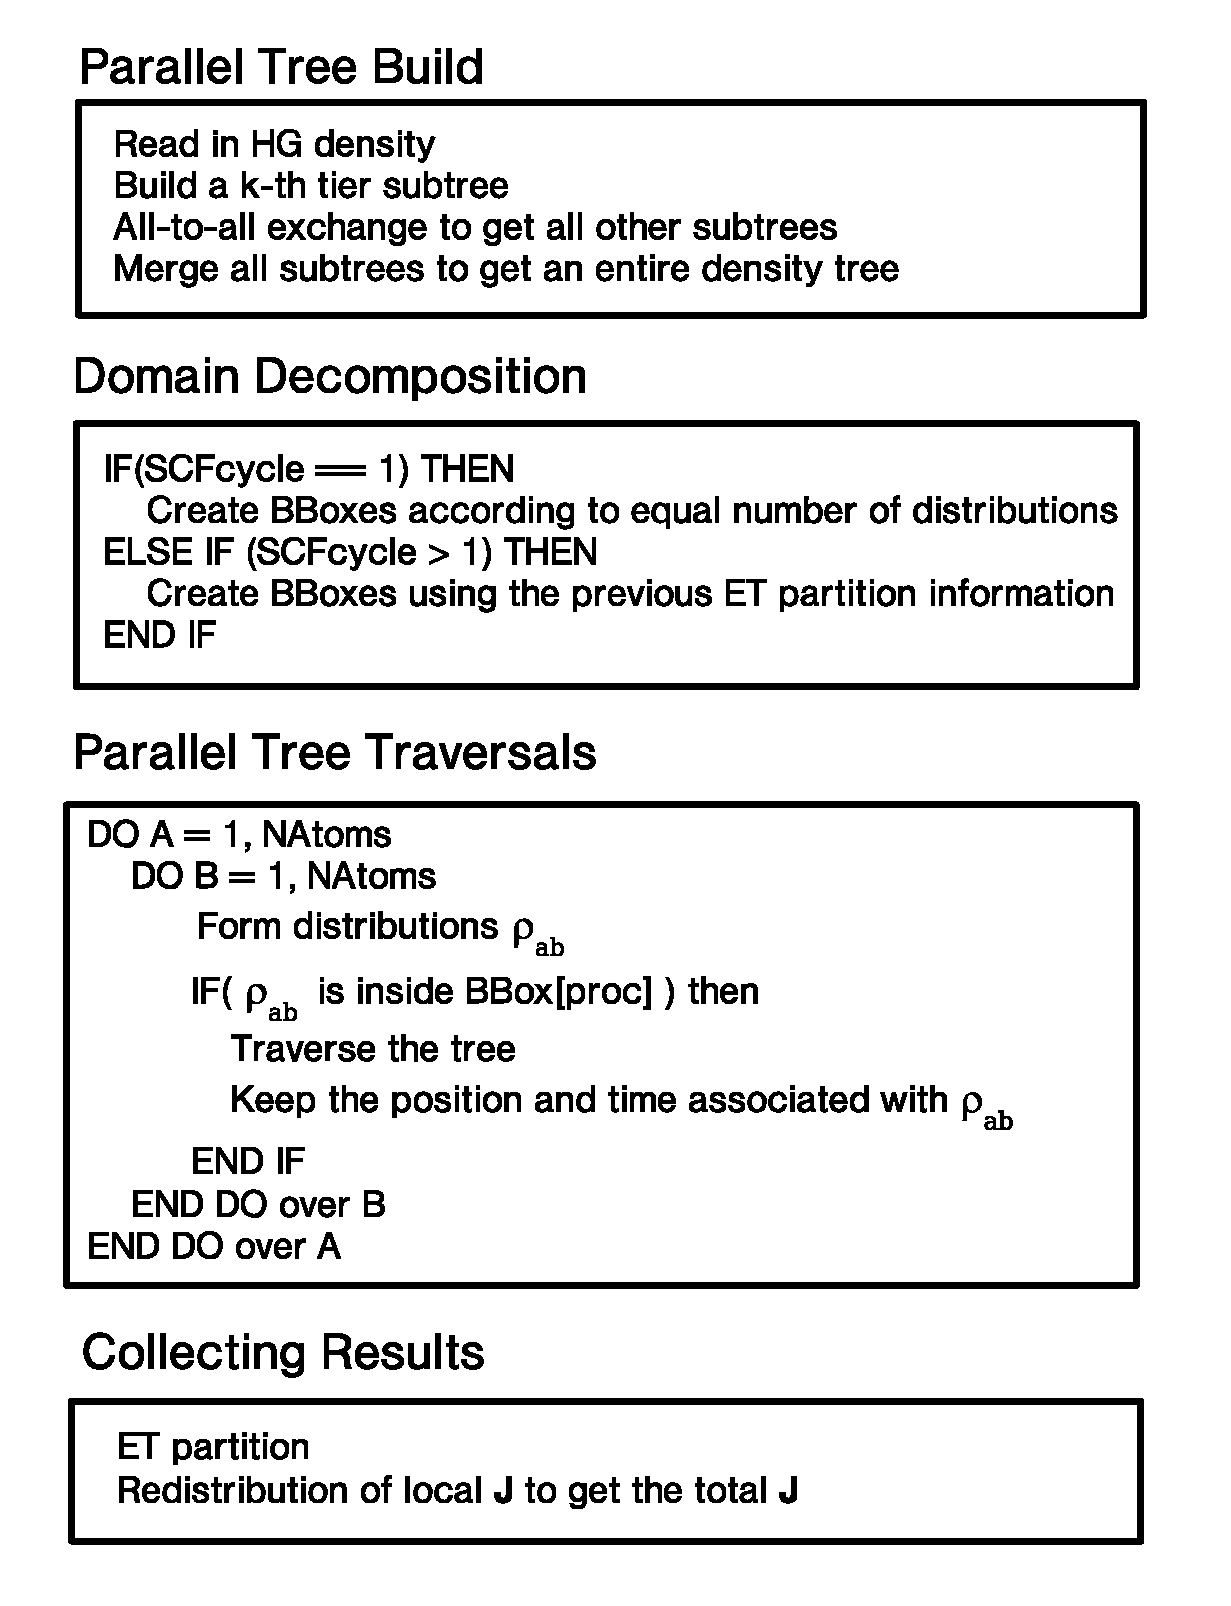
\includegraphics[clip]{pseudo.eps}}
\caption{ 
A pseudocode for parallel QCTC. Refer to the text for more details.
}
\label{fig:pseudo}
\end{figure}
}

\section{Implementation}
\label{sec:implementation}
We have implemented a parallel QCTC algorithm in {\sc
MondoSCF}~\cite{MondoSCF}, a suite of programs for linear scaling
electronic structure theory and {\it ab initio}\/ molecular dynamics.
Figure~\ref{fig:pseudo} shows the pseudocode for parallel QCTC.
It should be noted that the local and total Coulomb matrices are distributed,
while the entire density tree is replicated on all processors.
Thus the memory requirements are the same as in serial for the storage of
the density tree.
{\sc MondoSCF} has been written in Fortran 90/95 with the
message-passing library MPI~\cite{mpi}.  Timings are performed using
the {\tt MPI\_WTIME} function.

\section{Results}
\label{results}
We have performed scaling tests on both finite and periodic
systems. For the finite systems, we have chosen taxol
(C$_{47}$H$_{51}$NO$_{14}$) and 2 water clusters as test cases. For
the periodic systems, we have chosen pentaerythritol tetranitrate
(PETN)\cite{CGan04A} and the $\delta$-phase of
octahydro-1,3,5,7-tetranitro-1,3,5,7-tetrazocine
($\delta$-HMX)\cite{JPLewis00} as representative test cases. These
systems are chosen because they are inhomogeneous,
three-dimensional (and two are periodic) systems posing a challenge to
parallel QCTC. All runs were performed on a cluster of 256 4 CPU
HP/Compaq Alphaserver ES45s with the Quadrics QsNet High Speed
Interconnect.

For the purpose of performing the scaling tests, we start the
calculation with the STO-3G basis set and a low accuracy, switch
to the final basis set and accuracy using a mixed integral approach,
and run for three SCF cycles. The density matrix ${\bf P}$ is saved to
disk and scaling tests of parallel QCTC are performed. This procedure
may not be necessary. However, we are confident that the timings are
representatives of a routine calculation.

The result of the taxol scaling test is shown in Fig.~\ref{fig:taxol}.
The calculations are performed with the 6-31G and 6-31G** basis sets,
and a {\tt GOOD} accuracy\cite{CTymczak04a}.  The results of two
different speedups are presented.  The first speedup, called the ET
speedup, measures the efficiency of the ET partition for the Coulomb
matrix element calculation by traversing the density tree (see
Section~\ref{sec:ETPartition}) and is defined by
\begin{equation}
S_{ET} = \frac{2\tTT^{(2)}}{\tTT^{(n)}}
\end{equation}
where $\tTT^{(n)}$ is the time to evaluate the matrix elements by
traversing the density tree with $n$ processors. Notice that the
speedups are relative to a 2-processor calculation.  The second
speedup, called the QCTC speedup, measures the overall efficiency of
parallel QCTC. 
The timing for the QCTC speedup includes
reading in the HG density, building the 
density tree, traversing the density tree, ET partition for the 
next ${\bf J}$ calculation, and redistribution\cite{CGan03} of local ${\bf J}$ to realize 
the distributed total ${\bf J}$.
From Fig.~\ref{fig:taxol} it is observed that the ET
speedup is excellent up to 64 processors. 
Efficiencies at the
64-processor level (where the number of heavy atoms per processor is
less than 1) are 96.4\% and 94.5\% for the 6-31G and 6-31G** basis sets,
respectively. These efficiencies are better than that obtained using 
an equal-number-of-distributions partition (see Section~\ref{sec:ETPartition}),
where the efficiencies are 82.1\% and 79.0\% for the 6-31G and 6-31G** basis
sets, respectively.
% 60.46298
The overall parallel QCTC speedup is very good up to 32 processors but
degrades slightly at the 64-processor level.  The overall parallel
QCTC efficiencies at 64 processors are
% 49.64853 and 53.10910520061477
77.6\% and 83.0\% for the 6-31G and 6-31G** basis sets, respectively.

This loss of efficiency is due to the fact that the time for the parallel
density tree build does not decrease at the same rate (i.e.  divided
by the number of processors) as the tree traversal part.  In
Fig.~\ref{fig:time_ratio} we present the $\tTB/\tTT$ ratio as a
function of the number of processors for calculations on taxol (along
with other systems for comparisons to be made later).  We note that if
the time for parallel tree build $\tTB$ were to decrease at the same
rate as the time for tree
traversal $\tTT$ as we increase the number of processors, then the
$\tTB/\tTT$ ratio would remain constant.  However,
Fig.~\ref{fig:time_ratio} shows that the $\tTB/\tTT$ ratio increases
steadily as the number of processors is increased in all cases, a fact
that has been anticipated from the discussion in
Section~\ref{sec:parallelTB}.  Since the slope for the 6-31G** case is
smaller than that for the 6-31G case, this explains the slight
increase in the overall parallel QCTC performance of the 6-31G** case
over the 6-31G case, as shown in Fig.~\ref{fig:taxol}.

We note that our results of a parallel QCTC
% 7.7995003 and 7.772217865
speedup of 7.80 (with the 6-31G and 6-31G** basis sets) with 8
processors compares favorably with the speedup of about 6.0 of Sosa
{\it et al.}\cite{Sosa_00v26}, which is for an entire single-point
energy calculation with RHF/3-21G.

\commentoutA{
\begin{figure}[t]
\resizebox*{3.5in}{!}{\includegraphics[clip]{taxol-6-31g-6-31gss.eps}}
\caption{ 
Scaling of parallel QCTC on taxol (C$_{47}$H$_{51}$NO$_{14}$)
RBLYP/6-31G and RBLYP/6-31G**. Speedups are relative to a 2-processor
calculation.  The labels ET and QCTC denote equal time and overall
parallel QCTC speedups, respectively.  }
\label{fig:taxol}
\end{figure}
}

\commentoutA{
\begin{figure}[t]
\resizebox*{3.5in}{!}{\includegraphics[clip]{NProc_TTBTTTRatio.eps}}
\caption{ 
The ratio of the time to build the density tree ($\tTB$) to the time
to traverse the density tree ($\tTT$), as a function of the number of
processors.  }
\label{fig:time_ratio}
\end{figure}
}

\commentoutA{
\begin{figure}[t]
\resizebox*{3.5in}{!}{\includegraphics[clip]{sys1Iter2_sys2Iter3.eps}}
\caption{ 
Scaling of parallel QCTC on 2 cluster of water molecules with
RBLYP/6-31G**. Speedups are relative to a 2-processor calculation.  }
\label{110And200WaterOnGood}
\end{figure}
}

\commentoutA{
\begin{figure}[t]
\resizebox*{3.5in}{!}{\includegraphics[clip]{sys1Iter2_sys7Iter3.eps}}
\caption{ 
Scaling of parallel QCTC on 110-molecule water cluster with
RBLYP/6-31G** on {\tt GOOD} and {\tt TIGHT} accuracies.  Speedups are
relative to a 2-processor calculation.  }
\label{fig:110WaterOnGoodAndTight}
\end{figure}
}

\commentoutA{
\begin{figure}[t]
\resizebox*{3.5in}{!}{\includegraphics[clip]{NProc_TRatio_110H2O_GoodAndTight.eps}}
\caption{ 
The ratio of the time to build the density tree ($\tTB$) to the the
time to traverse the density tree ($\tTT$), as a function of the
number of processors, for 110-molecule water cluster (RBLYP/6-31G**)
calculations on {\tt GOOD} and {\tt TIGHT} accuracies.}
\label{fig:NProc_TRatio_110H2O_GoodAndTight}
\end{figure}
} 

Similar scaling tests have been performed on a 110-molecule and
200-molecule water clusters with RBLYP/6-31G** at a {\tt GOOD}
accuracy level.  The result of the scaling tests is shown in
Fig.~\ref{110And200WaterOnGood}. It is found that the ET speedups are
rather good for both cases. The overall parallel QCTC speedups are
% 80.31859859152611 and 85.53948967877915
80.3 and 85.5 for the 128-processor calculations for 110-molecule and
200-molecule water clusters, respectively.
%62.7\% and 66.8\% for the 110-molecule and 200-molecule 
The decrease in parallel QCTC efficiency is again due to the
% 28.80799713967989 and 26.56818727311716
high $\tTB/\tTT$ ratio at the 128-processor level. These ratios are
28.8\% and 26.6\% for the 110-molecule and 200-molecule water
clusters, respectively (see Fig.~\ref{fig:time_ratio}).

To investigate the performance of parallel QCTC at a higher accuracy
level, we have performed the scaling tests on a 110-molecule water
cluster but with {\tt TIGHT} accuracy\cite{CTymczak04a}. The results for both {\tt GOOD}
and {\tt TIGHT} accuracies are presented in
Fig.~\ref{fig:110WaterOnGoodAndTight} for comparison.  It is seen that
the ET speedup is better for the {\tt TIGHT} case than for the {\tt
GOOD} case. This is anticipated since increasing the accuracy level
increases the effective granularity, which leads to a better
performance in ET partition\cite{CGan03}.  Overall parallel QCTC
increases its efficiency from {\tt GOOD} to {\tt TIGHT}, which is due
mainly to a decrease in the $\tTB/\tTT$ ratio, as shown in
Fig.~\ref{fig:NProc_TRatio_110H2O_GoodAndTight}.


\commentoutA{
\begin{figure}[t]
\resizebox*{3.5in}{!}{\includegraphics[clip]{Sys3Iter3_Sys8Iter3.eps}}
\caption{ 
Scaling of parallel QCTC on $\delta$-HMX and PETN with RPBE/6-31G**.
Speedups are relative to a 2-processor calculation.  }
\label{fig:111DHMX212PETN}
\end{figure}
}

Finally, for the periodic systems, Fig.~\ref{fig:111DHMX212PETN} shows
that the overall parallel QCTC with RPBE/6-31G** at a {\tt GOOD}
accuracy level is excellent. At the 128-processor level, the $1\times
1\times 1$ $\delta$-HMX (168 atoms per simulation cell) delivers 104.0
fold speedup, while the $2\times 1 \times 2$ PETN (232 atoms per
simulation cell) delivers 100.0 fold speedup. These performances are
better compared to the 110-molecule (a speedup of 80.3) or
200-molecule (a speedup of 85.5) water cluster calculations. This is
due to the smaller $\tTB/\tTT$ ratio (see Fig.~\ref{fig:time_ratio})
for the periodic cases compared to the finite cases, which mainly
results from the increase in the time spent in the tree traversal part.
%(e.g. 87.7 and 64.0 secs for the $2\times 1 \times 2$ PETN and 200-molecule water cluster, respectively).

\section{Conclusions}
\label{conclusions}
We have proposed an efficient method of parallelizing linear scaling calculation of
the Coulomb matrix. The concept of equal time (ET) has proven fruitful
for load balancing the most time consuming part of QCTC, which is
traversal of the density tree for the matrix element calculation.
Equal time exploits the temporal locality between SCF iterations to
overcome strong spatial irregularities. It is expected that ET should
retain this property between geometry steps in an optimization or
molecular dynamics run.  The efficiency of the ET partition ranges
from 91 -- 98 \% for all test cases presented in this work at the
128-processor level. The overall QCTC speedup, however, ranges from 63
-- 81 \% overall efficiency at the 128-processor level with fine
grained parallelism.  The decrease in efficiency is mainly due to the
parallel tree build process.  While the current simple implementation
of the parallel tree build should eventually be replaced by a more
sophisticated version, the current implementation has enabled us to
run routine calculations to address a range of interesting
problems\cite{CGan04A,CGan04C}.

\begin{acknowledgments}
This work has been carried out under the auspices of the
U.S. Department of Energy under Contract No.~W-7405-ENG-36 and the
ASCI project.  Most work was performed on the computing resources at
the Advanced Computing Laboratory of Los Alamos National Laboratory.
\end{acknowledgments}

\bibliographystyle{apsrmp} \bibliography{mondo_new}

\end{document}
